\section{Interface Descriptions}
While it may seem far removed from the core programming aspect of software engineering, the design of a good user interface is key to the success of any system. Indeed, Douglas Bell (1987) went so far as to claim that the user interface is the “yardstick by which a system is judged,” and certainly it plays a crucial role in attracting users to the software.

This section will describe what factors are taken into consideration in the design of the interface for the Fortitude application, and how the final product will be suitable, appealing and fulfil the criteria set forth in the requirements document (23 Cats, 2012).

\subsection{Design Methodology}

\begin{wrapfigure}{l}{0.2\textwidth}
	\vspace{-20pt}
	\begin{center}
	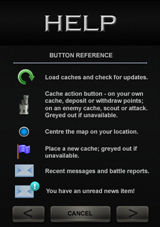
\includegraphics[width=0.2\textwidth]{images/interface1}
	\caption{Button reference in the help}
	\end{center}
	\vspace{-10pt}
\end{wrapfigure}

While designing the interface, it was important at all times to consider ease of use for users of various levels of familiarity with the system. Our domain analysis had highlighted the importance of intuitiveness in a system and of required functions being easily accessible (23 Cats, 2012:5-7); for this reason we have tried at all times to make the interface clear, and have also included a help screen should the user ever require it (see fig 2.1). Bell (1987) highlights the role of a well designed user interface in reducing errors, and to this end several of the features of our app were tested on potential users during development. In particular, it had originally been decided to disable the android back button within the app to give us greater control over which screens the user could access at any point in time. However, our users found the lack of a back button difficult to get used to, and so its functionality has been incorporated into the application wherever possible.

To further the ease of use of the Fortitude Application, buttons which perform a specific action will be greyed out when the action is not available. These include, for example, the ‘place cache’ button which would be greyed out if the user was too close to an existing cache, shown right in fig 2.2. The greyed out flag would

\begin{tabular}{| p{0.22\textwidth} | p{0.68\textwidth} |}
	\hline
	\vspace{10mm}
	Caches & \lipsum[1] \\
	\hline
	\vspace{10mm}
	Users & \lipsum[2] \\
	\hline
\end{tabular}
